\documentclass[12pt]{article}
\usepackage{amsmath}
\usepackage{physics}
\usepackage{amssymb}
\usepackage{graphicx}
\usepackage{hyperref}
\usepackage{amsfonts}
\usepackage{cancel}
\usepackage{xcolor}
\hypersetup{
	colorlinks,
	linkcolor={black!50!black},
	citecolor={blue!50!black},
	urlcolor={blue!80!black}
}
\newcommand{\f}[2]{\frac{#1}{#2}}
\usepackage{newpxtext,newpxmath}
\usepackage[left=1.25in,right=1.25in,top=1.25in,bottom=1.25in]{geometry}
\usepackage{framed}
\usepackage{caption}
\usepackage{subcaption}


\usepackage{cite} %Imports biblatex package




\begin{document}
\begin{framed}
\begin{center}
{\large PH312: Physics of Fluids (Prof. McCoy) -- Final Paper}\\
{ Huan Q. Bui}\\
\today
\end{center}
\end{framed}



\begin{center}
	\Large{\textbf{Leonardo's Obsession}}
\end{center}



The advent of modern computing has allowed scientists to study turbulence with an unprecedented level of detail. One needs to look no further than the ubiquitous streamlined look of modern skyscrapers or the increasingly advanced technology in speed sports (e.g. sailing, swimming, cycling, and so on) to find computer-assisted designs with aims to ``tame'' turbulence. Do these designs work? Absolutely. Fantastically, in fact. Humans have redirected rivers, sent other humans to the Moon and back, and are traveling faster and much more efficiently than ever before -- all thanks to our ability to deal with turbulence and utilize various properties of fluid motion at large. Yet, we have not really \textit{understood} turbulence. We don't know how or when turbulence may occur, and we are obsessed with trying to understand turbulence, so much so that we have a million-dollar prize for the first person to solve the notorious Navier-Stokes Equation -- arguably the key to all of fluid dynamics. Richard Feynman famously said: ``Turbulence is the most important unsolved problem of classical physics,'' and he is probably right!  \\

When did our obsession with turbulence start? On the one hand, one may argue that it began in the 18th century with the rise of Reynolds, Raleigh, Kelvin, Helmholtz, and so on, who were not only brilliant scientists but also equipped with the power of calculus. They were the pioneers of fluid dynamics as we know it today: many important dimensionless quantities, partial differential equations, and phenomena in hydrodynamics bear their names.  On the other hand, one may travel way back to antiquity and argue that the obsession with turbulence -- or \textit{chaos} -- had already begun then, hidden in Greek mythology and creation stories across civilizations. One may also find a middle ground: in fact we can perhaps argue that our obsession with turbulence started sometime between these chronological extremes -- during the High Renaissance -- due to an Italian polymath named Leonardo da Vinci (1452 -- 1519). Through his innumerable drawings and verbal collections, one find it evident that hydrodynamics (especially turbulence) was da Vinci's lifelong obsession, and he made sure that, 500 years later, his obsession becomes ours \cite{lavin1993leonardo}. \\



Keeping in mind that there was no calculus (and thus no differential equations) at his time, we see Leonardo da Vinci's genius through his categorization of flow in his studies, many of which modern classification of flows resemble -- half a millennium later! A prime example is shown in Figure \ref{fig:1}. The first sketch shows currents and counter-currents, which occur when currents cross each other. The second sketch shows flow over a irregular surface, illustrating that water flows faster at the surface than down below near the bottom (velocity gradient!). The third sketch shows water falling off a cliff and how an object at the drop may remain there in a stable position. The fourth sketch is similar to the second sketch -- illustrating the idea of a velocity gradient in which the flow near the boundary is slower than in mid-stream.  Figure \ref{fig:5} shows his study of water flowing out of a pipe in comparison to the outflow of blood from the aorta -- a canonical case study in modern fluid dynamics. He wrote: ``The water that rises through a pipe, that which rises highest will be furthest away from the walls of the pipe.'' -- a very keen observation from today's fluid dynamical standpoint.  Leonardo da Vinci also studied flow around an obstacle and made a number of other remarkable observations regarding vortices and wake formations. An example is given in Figure \ref{fig:2} \cite{marusic2021leonardo}. \\



\begin{figure}[!htb]
	\begin{subfigure}{0.45\textwidth}
		\centering
		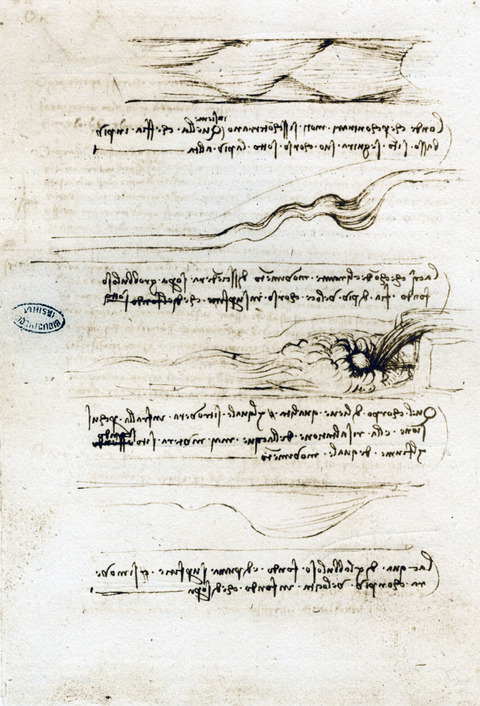
\includegraphics[height=0.4\textheight]{LdV_1}
		\caption{Leonardo da Vinci, movement of water, ca. 1492. Paris, MS. A, fol. 24v.}
		\label{fig:1}
	\end{subfigure}
\hspace{10pt}
	\begin{subfigure}{0.45\textwidth}
		\centering
		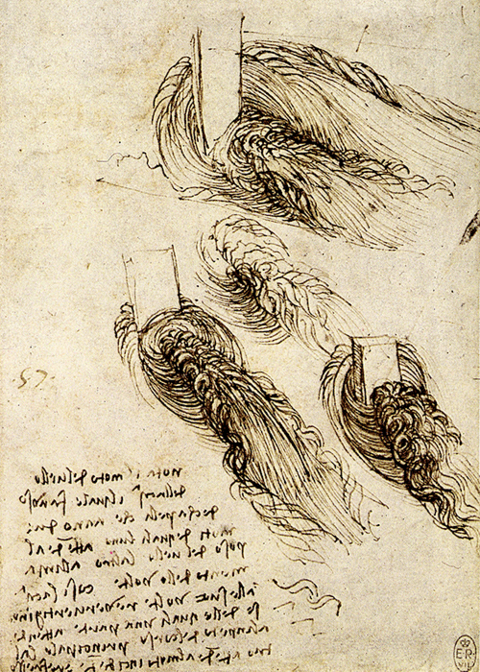
\includegraphics[height=0.4\textheight]{LdV_2}
		\caption{Leonardo da Vinci, movement of water, ca. 1513.  Windsor, Royal Library, 12579r, detail.}
		\label{fig:2}
	\end{subfigure}
\end{figure}


\begin{figure}[!htb]
	\centering
	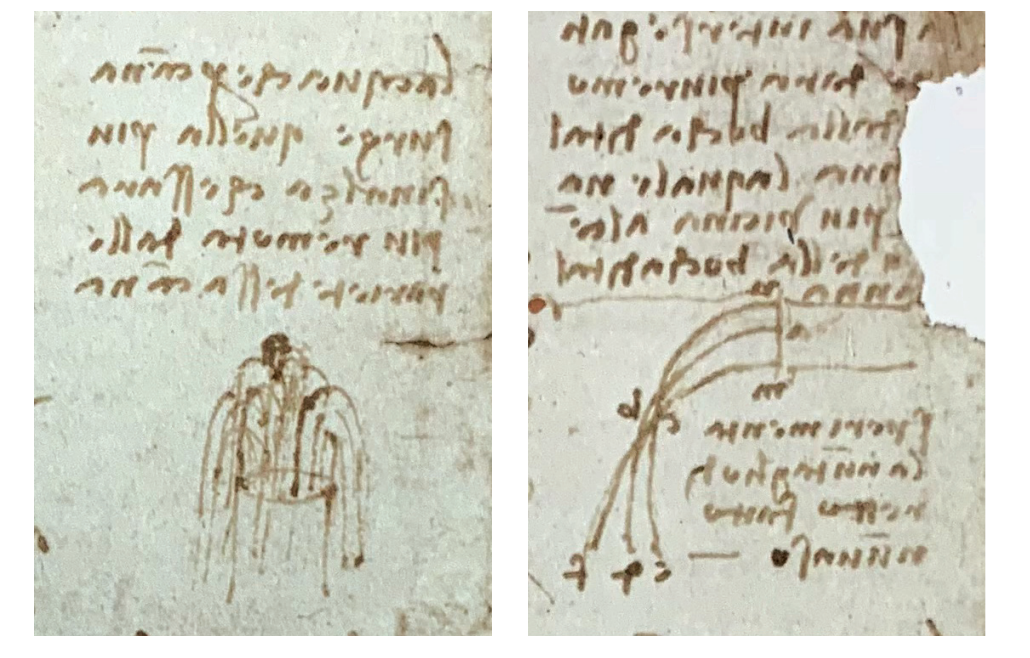
\includegraphics[width=0.8\textwidth]{LdV_5}
	\caption{Pipe flows showing a varying velocity gradient. Royal Collection at Windsor (RCIN 919117r).}
	\label{fig:5}
\end{figure}





Given his genius, it is not surprising to find that Leonardo da Vinci foreshadowed many concepts used in the modern study of turbulence. He used the word \textit{turbolenza} in many of his writings, in both the technical sense as we know today and the more anthropomorphic sense to describe ``raging movement of water'' \cite{marusic2021leonardo}. da Vinci was obsessed with turbulence, especially toward the end of his life. This obsession resulted in a collection of his drawings, called the \textit{deluge drawings}, in which he captured in spectacular detail all the small and large eddies and currents and counter-currents in turbulent, boiling water. Figures \ref{fig:3} and \ref{fig:4}, among many others, show an example of the extreme meticulousness. Interestingly, Leonardo da Vinci's  point in making these drawings was to depict the cataclysmic biblical events, and in trying to do so in the most realistic way he became a master of drawing turbulent flows. da Vinci wrote about his approach to visualizing turbulence: ``The swollen waters will swirl around the pool that
encloses them, striking with dizzying eddies against the different objects, and throwing out into the air muddy foam, then falling back, making the beaten water refract in the air'' (RCIN 912665), showing that he was highly aware of the distinctions between various forms of the  water's movement \cite{marusic2021leonardo}. \\



\begin{figure}[!htb]
	\begin{subfigure}{0.49\textwidth}
		\centering
		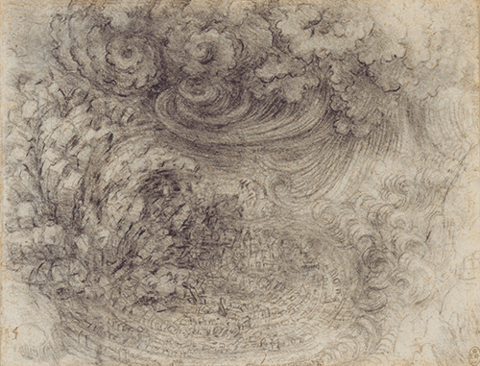
\includegraphics[width=0.9\textwidth]{LdV_3}
		\caption{Leonardo da Vinci, Deluge, ca. 1512-16.  Windsor, Royal Library, 12378.}
		\label{fig:3}
	\end{subfigure}
	\begin{subfigure}{0.49\textwidth}
		\centering
		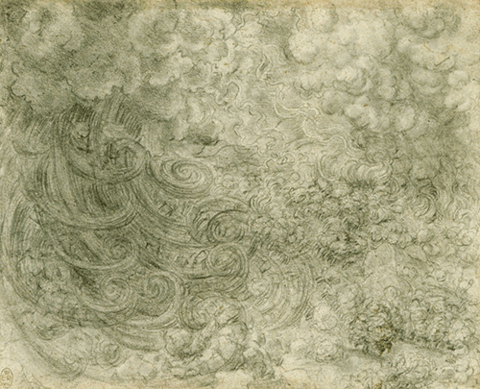
\includegraphics[width=0.84\textwidth]{LdV_4}
		\caption{Leonardo da Vinci, Deluge. Windsor, Royal Library, 12384.}
		\label{fig:4}
	\end{subfigure}
\end{figure}
 
Figure \ref{fig:6} is perhaps one of da Vinci's most famous depictions of turbulent flow. Figure \ref{fig:6}a shows water being poured strongly into a pool, resulting in turbulence with air bubbles and eddies interacting at various scales. Figures \ref{fig:6}b, c show the development of turbulence, from the same ``experimental setup,'' clearly showing that da Vinci was thinking about {vortices} and their roles in the birth and description of turbulence. What's amazing about these drawings (apart from the fact that they are so realistic), is that they were constructed out of da Vinci's imagination. Keep in mind that there was no high-speed photography in Leonardo's time (The first attempt to capture an image using a camera obscura and silver nitrate was in the early 1800s, 300 years after da Vinci's time), and it is not possible to ``freeze'' the movement of water -- turbulence and vortices are in constant motion and evolution. As a result, these drawings we see are not snapshots of turbulence, but rather are Leonardo da Vinci's \textit{interpretative syntheses} of the phenomenon \cite{marusic2021leonardo}. Here, we emphasize the phrase ``interpretive syntheses'' because da Vinci did not appear to simply create these drawings photographically from memory. Rather, careful analysis shows that the eddies and vortices in these drawings aren't just random curves that da Vinci jotted down; they are actually well-approximated by self-similar logarithmic curves! It also turns out that there is a power-law associated with the spatial distribution of the eddies, suggesting that the patterns in his drawings are intentional \cite{marusic2021leonardo}. It is thus clear to us that Leonardo da Vinci was trying to understand or figure out some universal law governing turbulence, and we see why he was a polymath who observed the natural world and theorized possible explanations for phenomena which he did not understand, rather than an artist who recreated and re-rendered these phenomena only for illustration's sake.\\



\begin{figure}[!htb]
	\centering
	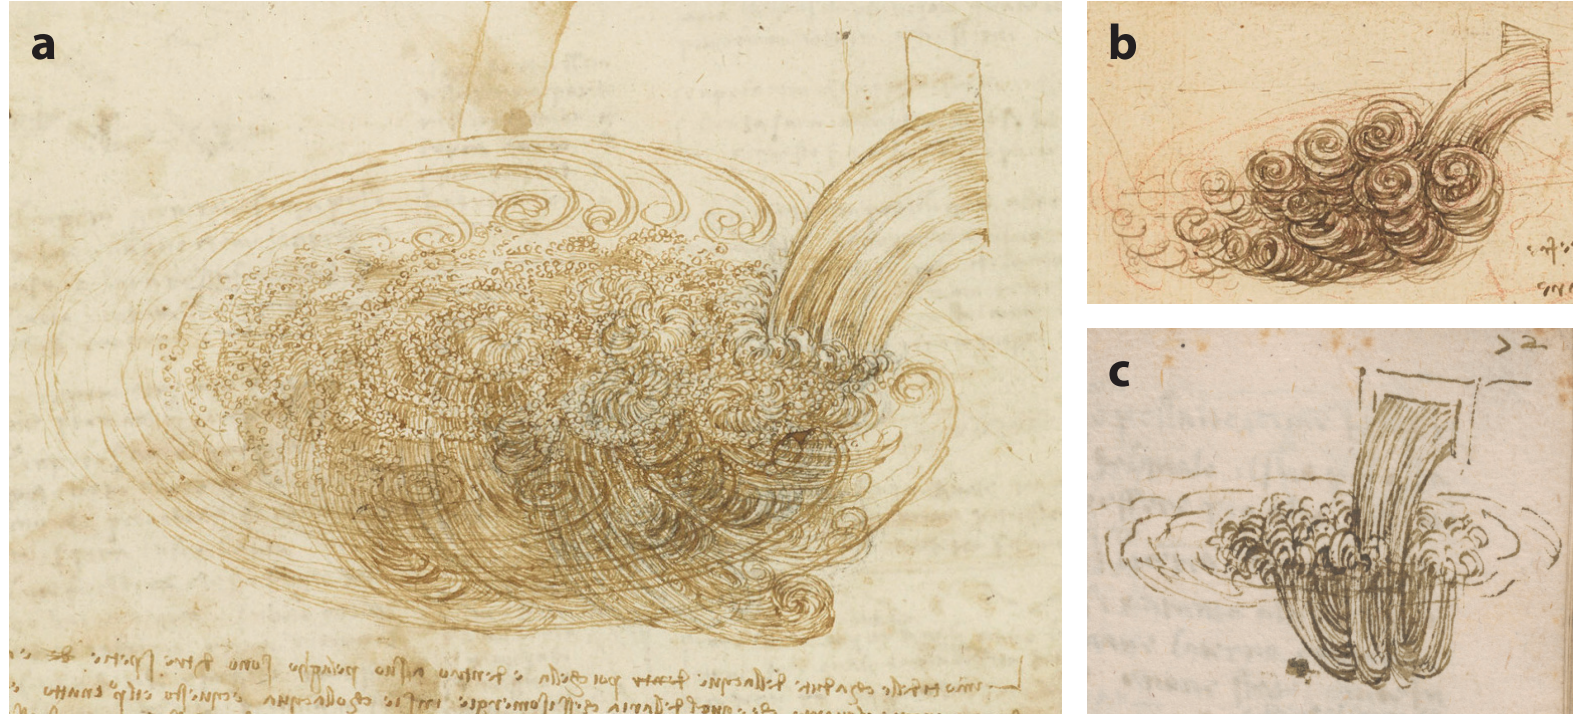
\includegraphics[width=0.95\textwidth]{LdV_6}
	\caption{Sketches of a plunging water jet into a pool, with the resultant turbulent flow. (a) RCIN 912660v, (b) RCIN 912662, (c) RMN-Grand Palais (Institut de France)}
	\label{fig:6}
\end{figure}



While many of the complexities which Leonardo da Vinci tried to capture in his drawings of water movement were well beyond his reach (some of these complexities are still beyond the reach of modern mathematics and physics), I still think he had added tremendous value to our understanding of turbulence and fluid dynamics at large. At the very least, he had created beautiful and highly artistic work. Besides the detailed accounts of his observations of fluid dynamical phenomena, I think the fact that a genius like da Vinci considered fluid motion interesting alone was more than sufficient to inspire, directly or indirectly, scientists of later generations to also study the subject. The most notable example is perhaps Isaac Newton, who is famously known today for his invention of calculus (alongside Leibniz) and the formulation of classical mechanics. Unbeknown to most of us, Newton spent a great deal of his life studying \textit{drag forces} \cite{smith1998newton}.  He also conceived novel ideas such as \textit{Newtonian fluids}, \textit{viscosity}, and various types of \textit{stress} and studied the flow of water from orifices and many wave phenomena. And as we know, following Newton, we have the familiar names of Reynolds, Kelvin, Helmholtz, and so on. By tracing everything back to da Vinci's time, we see that fluid dynamics has a deeply rooted history, a history as deep as the history of development of physics and mathematics and the natural sciences themselves. It is a history which perhaps began when Leonardo da Vinci planned to divert the river Arno away from Pisa and dreamed of machines that could fly, a history which might have originated from Leonardo's obsession with something as seemingly trivial and ordinary as the movement of water.





\bibliographystyle{unsrt}
\bibliography{fluids}
\end{document}




